\documentclass{article}
\usepackage[margin=1in]{geometry}

\usepackage{amsmath,graphicx}

\title{TDSE Code - User Guide, Best Practices, and Developers Notes}
\author{J. Venzke}

\begin{document}
\maketitle

\tableofcontents
\newpage

\section{Introduction} % (fold)
\label{sec:introduction}
\subsection{Code Overview} % (fold)
\label{sub:code_overview}
The TDSE code discussed here was mainly developed by Joel Venzke while working on his Ph.D. in the Ultrafast Theory Group in JILA. Cory Goldsmith and other group members have also contributed to this code in various forms. It solves the Time Dependent Sch\"{o}dinger Equation (TDSE) for various targets in a laser field with for single active electrons. It has support for two or more active electrons, but the computational power of modern super computers limits the calculation that are possible to 2 electrons in 2 spacial dimensions. For single active electrons, I have developed a cylindrical 2D code for linear polarized light. All other calculations requirer use of the Cartesian grid code. Future work will look to push towards a 2 electron full 6D code, and extending the code to different coordinate systems/basis methods.

This code has support for real space propagation of the TDSE using finite differences for spacial derivatives and Crank-Nicolson for time propagation. The codes has been shown to scale out to 6,000+ processors (we ran out of computer). It can also simulate interesting physics on a laptop if you have a few hours of free time. The main drive for developing this code is to push simulations passed the current limit.
% subsection code_overview (end)

\subsection{Problems of interest} % (fold)
\label{sub:problems_of_interest}
At the attosecond ($10^{-18} seconds$) time scale, molecular motion is frozen, and electron dynamics dominate all processes. In order to study how electrons interact with attosecond laser pulses, we solve the Time-Dependent Sch\"{o}dinger Equation (TDSE). This can be done relatively easily for 1 electron with linear polarized light, however, circular polarization and multi-electron effects make the calculations more computationally interesting. Gaining a deeper understanding the behavior of electrons induced by intense ultrashort laser pulses is the reason this code was developed.
% subsection problems_of_interest (end)


\subsection{Development Goals} % (fold)
\label{sub:development_goals}
This code is being designed with large scale numeric simulation in mind. We want to be limited by the largest computer we can get our hands on, not the fastest desktop on the market. That being said, for small scale simulation, there are better more efficient codes. However, those codes will reach limitations due to hardware which is where a large scale code like this starts to shine. For that reason, MPI is used for parallelization so that we can utilize HPC systems.

Since this code is for physics, we want the users to be able to focus on physics rather than the computer science back end. As a result, the pipe dream is to have all simulations only require an input file with no need to write code. It maybe necessary to learn python for custom data visualizations, but many of the visualizations needed to analysis the results are included with the repo. You may also need to implement small c++ changes if you wish to simulate targets that do not fit the current layout or various other unsupported tasks, though I hope to make this code relatively general.

It would also be nice that when the simulation is complete, the code produces enough plots to make sure that the simulation worked and a basic overview of the interesting physics the simulation contains. For this reason, all visualization is done in a batch mode and images are saved in a ``figs'' directory.

Finally, we want this code be useful in future iterations. Therefor we used GitHub for version control. We are also working on in source documentation to ease development efforts.
% subsection development_goals (end)

\subsection{Key Features} % (fold)
\label{sub:key_features}

% subsection key_features (end)
% section introduction (end)

\section{Running TDSE and Best Practices} % (fold)
\label{sec:running_tdse_and_best_practices}

% section running_tdse_and_best_practices (end)

\section{Theory} % (fold)
\label{sec:theory}

The TDSE can be written simply as
\begin{equation}
    i\frac{\partial}{\partial t}\psi(x,t) = \hat{H}\psi(x,t)
\end{equation}
In the velocity gauge the Hamiltonian becomes
\begin{equation}
    \label{eq:atoms_and_molecules}
    \hat{H} = \sum_{e}\left(\frac{\hat{\mathbf{p}}^2_e}{2} - \frac{\mathbf{A}(t) \cdot \hat{\mathbf{p}}_e}{c} - \sum_{n} \frac{Z_n}{r_{e,n}}\right) + \sum_{e_1 < e_2}\frac{1}{r_{e_1, e_2}}
\end{equation}
\begin{itemize}
    \item $\hbar=e=m=1$ (atomic units)
    \item $\hat{H}$ is the Hamiltonian
    \item $\hat{\mathbf{p}}$ is the momentum operator $(-i\nabla)$
    \item $\mathbf{A}(t)$ is the vector potential that describes the laser
    \item $c$ is the speed of light (137ish in a.u.)
    \item $Z_n$ is the nuclear charge
    \item $r_{i,j}$ is the Euclidean distance between $i$ and $j$
\end{itemize}
This Hamiltonian assumes that the wavelength is much larger than the radius of the atom (dipole approximation), the field has a large number of photons (it treats fields classically), and the nuclei are fixed in space during the simulation (molecular motion is much slower than electron motion). Moving (classically and quantum mechanically) nuclei are on the wish list for this code.

The first term in Equation~\ref{eq:atoms_and_molecules} is the kinetic energy of the electron. In atomic units, this can be written such that
\begin{equation}
  \frac{\hat{\mathbf{p}}^2_e}{2} = \frac{\nabla_e^2}{2}
\end{equation}
Note that the subscript $\nabla_e^2$ means the derivatives only act on the $e$th electron and acts like the identity operator on all other electrons.

The second term is the laser electron interaction.
\begin{equation}
  - \frac{\mathbf{A}(t) \cdot \hat{\mathbf{p}}_e}{c} = \frac{\mathbf{A}(t) \cdot i\nabla_e}{c}
\end{equation}
The laser is given as a vector potential. A short discussion on that is provided in Section~\ref{sub:lasers}.

The third term is the Coulomb potential for each nuclei.
\begin{equation}
  - \sum_{n} \frac{Z_n}{r_{e,n}}
\end{equation}
This is often implemented with a soft core (Section~\ref{ssub:soft_core_like}) to avoid the singularity at $r_{n,e}=0$ though this is not required for full 3D simulations. Some reviewers are not a fan of soft cores, so be careful when deciding to use them. The code allows for any locations for atomic targets. This allows any molecule to be implemented in the code without the need to recompile. You can also add frozen electrons to a nuclei using single active electron potentials found in Section~\ref{ssub:single_active_electron}.

The last term is the electron electron coloration term.
\begin{equation}
  \sum_{e_1 < e_2}\frac{1}{r_{e_1, e_2}}
\end{equation}
It gives the repulsion of the electron with all other electrons. This is the term that couples every electron in the system and leads to an N electron calculation becoming a 3N dimensional Hilbert space leading to 2 electron simulations being the biggest we can hope to simulate with current computing technologies. If you neglect this term and put it into some effective potential, you can get either a TDDFT type calculation (not supported in this code) or a single active electron potential depending on how you do it.

\subsection{Spacial Derivatives} % (fold)
\label{sub:spacial_derivatives}
For spacial derivatives, this code utilized finite differences (though other methods are being implemented). When using finite differences, derivatives can represented by a set of coefficients called a stencil. The stencil provides the non-zero $c_i$ weights for various sample points of the function. You can then write the second derivative of $\psi$ known at various evenly spaced grid points labeled by $n$ as
\begin{equation}
    \frac{d^2}{dx^2}\psi_n = \frac{1}{\Delta x^2}\sum_i c_i \psi_i
    \label{eq:finite_diff}
\end{equation}
The non zero $c_i$ coefficients are given in the table below for various orders of accuracy.
\begin{center}
\begin{tabular}{ |c|c|c|c|c|c|c|c| }
\hline
Order & $c_{n-3}$ & $c_{n-2}$ & $c_{n-1}$ & $c_{n}$ & $c_{n+1}$ & $c_{n+2}$ & $c_{n+3}$ \\ \hline
2nd   &      &      & -1   & 2  & -1   &      &      \\ \hline
4th   &      & $-\frac{1}{12}$ & $\frac{4}{3}$   & $-\frac{5}{2}$  & $\frac{4}{3}$   &  $-\frac{1}{12}$    &      \\ \hline
6th   &   $\frac{1}{90}$   &  $-\frac{3}{20}$    & $\frac{3}{2}$   & $-\frac{49}{18}$  & $\frac{3}{2}$   &   $-\frac{3}{20}$    &   $\frac{1}{90}$  \\ \hline
\end{tabular}
\end{center}

For the remainder of this discussion, we will assume we are using second order derivatives. However, this will be expendable to higher order derivatives by adding more off diagonal elements in matrices we will discuss in this section.

For the start of this discussion, we will consider a 1D wavefunction. We will later extend this to ND wavefunctions. We start with $\psi(x)$ known at various points along the $x$ axis spaced by a grid step of $dx$. We will label the points by $n$ such that $\psi_n = \psi(x_0 + dx*n)$ with $x_0$ being the lowest $x$ value. Plugging this into Equation~\ref{eq:finite_diff} we get
\begin{equation}
    \frac{d^2}{dx^2}\psi_n = \frac{1}{\Delta x^2}\left(-\psi_{n-1}+2\psi_n-\psi_{n+1} \right)
    \label{eq:finite_diff_second_order}
\end{equation}
Now we can write this for the point $\psi_{n+1}$ giving us
\begin{equation}
    \frac{d^2}{dx^2}\psi_{n+1} = \frac{1}{\Delta x^2}\left(-\psi_{n}+2\psi_{n+1}-\psi_{n+2} \right)
    \label{eq:finite_diff_second_order_n+1}
\end{equation}
This can be done until we hit the other end of the grid. If we take the boundary condition that $\psi(x_0-dx)=0$ and likewise on the other end, we can write our operator as a system of linear equations in the form of a matrix. Our matrix becomes
\begin{equation}
\frac{d^2\psi}{dx^2} =
\frac{1}{\Delta x^2}
\begin{bmatrix}
    2 & -1 &  &  &   &  \\
    -1 & 2 & -1 &  &  &  \\
     & \ddots & \ddots & \ddots & \\
     &  & -1 & 2 & -1\\
     &   &  & -1 & 2
\end{bmatrix}
\begin{bmatrix}
    \psi_{0} \\
    \psi_{1} \\
    \vdots  \\
    \psi_{N-1}  \\
    \psi_{N}
\end{bmatrix}
\end{equation}
One then uses a tensor product to produce the 2 and 3 dimensional versions.
% subsection spacial_derivatives (end)

\subsection{Time Propagation} % (fold)
\label{sub:time_propagation}
Time propagation is often performed using the split-operator method where the Hamiltonian ($\hat{H}$) split into its spatial dimensions, e.g. along ($z$) and perpendicular ($\rho$) to the laser polarization direction. The resulting propagation scheme is
%
\begin{equation}
    \psi(\mathbf{r},t+\Delta t) \approx e^{-i\hat{H}_{\rho}\frac{\Delta t}{2}} e^{-i\hat{H}_z(t)\Delta t} e^{-i\hat{H}_{\rho}\frac{\Delta t}{2}}\psi(\mathbf{r},t).
     \label{eq:Split-operator}
\end{equation}
%
where
\begin{equation}
    e^{-i\hat{H}\Delta t} \approx \frac{1-i\frac{\Delta t}{2} \hat{H}}{1+i\frac{\Delta t}{2} \hat{H}}
\end{equation}
produces a set of tridiagonal matrices which can be solved with $\mathcal{O}(\mathcal{N})$ operations and $\mathcal{O}(\mathcal{N})$ memory. However, parallelization of such a method on a modern supercomputer with distributed memory can be cumbersome, requiring multiple all-to-all Message Passing Interface (MPI) messages during each time step.

Instead, we avoid splitting the Hamiltonian and propagate the total Hamiltonian in time using a second order Crank-Nicolson scheme where
%
\begin{equation}
    \psi(\mathbf{r},t+\Delta t) \approx e^{-i\hat{H}\Delta t}\psi(\mathbf{r},t).
    \label{eq:Crank_Nicolson}
\end{equation}
%
We note that the Crank-Nicolson method is not tridiagonal (due to a tensor product) and a direct solution would require $\mathcal{O}(\mathcal{N}^3)$ operations and $\mathcal{O}(\mathcal{N}^2)$ memory which is significantly more than in the split operator method. However, the system of equations in the full Crank-Nicolson method is sparse and iterative methods can be used to vastly accelerate the time propagation. We utilize the Generalized Minimal Residual Method (GMRES), implemented in PETSc, which solves the sparse system of linear equations in $\mathcal{O}(\mathcal{N}\log(\mathcal{N}))$ operations and $\mathcal{O}(\mathcal{N})$ memory. The PETSc library makes it straightforward to parallelize the Crank-Nicolson method on modern supercomputers with distributed memory. On a local supercomputer (Summit, CU Boulder), we achieved super-linear scaling up to 3,000+ cores allowing us to complete simulations in a matter of hours that would take weeks running on a high-end workstation.

\subsubsection{Exterior Complex Scaling (ECS)} % (fold)
\label{ssub:exterer_complex_scaling}
To absorb any outgoing wave packets, we utilize an exterior complex scaling (ECS). This is equivalent to changing the spacial step used in finite difference from $x_{n+1} = x_n+dx$ to $x_{n+1} = x_n+e^{i\eta}dx$ where $\eta=\pi / 4.0$ seams to work well. This leads to an exponential decay of the wavefunction in the absorbing region.

% subsubsection exterer_complex_scaling (end)
% subsection time_propagation (end)

\subsection{Atoms and Molecules} % (fold)
\label{sub:atoms_and_molecules}
The code allows for nuclei to be placed at any location assuming the coordinate system supports it. This allows for molecular targets to be build by hand with each nuclei having a unique potential. The potentials available are laid out below.

\subsubsection{Soft Core} % (fold)
\label{ssub:soft_core_like}
A soft core can be used to calculate distances. This removes the singularity of the coulomb potential, however, reviewers are often not a fan of such a method. Use a soft core only when required. The soft core is calculated using
\begin{equation}
  r_{soft} = \sqrt{r^2 + \alpha^2}
\end{equation}
where $r$ is the euclidean distance and $\alpha$ is the soft core parameter.
% subsubsection soft_core(end)

\subsubsection{Hydrogen Like} % (fold)
\label{ssub:hydrogen_like}
The code provides a coulomb potential with the form
\begin{equation}
  V(r) = -\frac{Z}{r}
\end{equation}
where $Z$ is the nuclear charge and $r$ is the euclidean distance (or soft core if $\alpha \ne 0$)
% subsubsection hydrogen_like (end)

\subsubsection{Single Active Electron} % (fold)
\label{ssub:single_active_electron}
Single active electron (SAE) potentials allow for a multi electron system, such as Helium, to be approximated by studying on active electron. The potentials available in this code take the form:
\begin{equation}
  V(r, r_{soft}) = - \frac{c_0}{r_{soft}} - \frac{Z_c e^{-r_0 r}}{r_{soft}} - \sum_n a_n e^{-b_n r}
    \label{eq:SAE}
\end{equation}
where $r_{soft}$ is the soft core distance from the nuclei's location and $r$ is the euclidean distance form the nuclei's location. Talk to Brynn or I to get parameters for different targets.

I would like to make this a tad more general.
% subsubsection single_active_electron (end)
% subsection atoms_and_molecules (end)

\subsection{Lasers} % (fold)
\label{sub:lasers}

To ensure a laser is ``physical'', it is required that the electric field ($E(t)$) integrates to zero. The easiest way to handle this is to set the vector potential directly ($A(t)$) and calculate $E(t)$ such that
\begin{equation}
A(t) = \frac{cE_0}{\omega_A} f(t) \sin(\omega_A(t-\tau_0)+\phi_A)
\label{eq:afield}
\end{equation}
and
\begin{equation}
\begin{split}
\label{eq:efield}
E(t) =& -\frac{1}{c}\frac{\partial}{\partial t}A(t)
\\
=&-E_0f(t) \cos(\omega_A (t-\tau_0) +\phi_A)
\\
&
+\frac{E_0}{\omega_A}\frac{\partial f(t)}{\partial t}
\sin(\omega_A (t-\tau_0) +\phi_A).
\end{split}
\end{equation}
$f(t)$, $\omega_A$,
$c$, $E_0$, $\tau_0$, and $\phi_A$ are the envelope function, central frequency of the vector potential, speed of light, amplitude of the electric field, the time the carrier envelope phase is set, and carrier envelope field (CEP) of the vector potential respectively. The central frequency of the electric field $\omega_E$ is the important one. To set is one must correct for it in $\omega_A$ using the following relation
\begin{equation}
\label{eq:fshift}
\frac{\omega_E}{\omega_A} = \frac{1+\sqrt{1+\mu/N^{2}}}{2}
\end{equation}
with N being the number of cycles in $\tau$ of the envelope. For the sine squared
\begin{equation}
f(t) = \sin^2\left(\frac{\pi t}{\tau}\right)
\label{eq:sin2}
\end{equation}
and Gaussian
\begin{equation}
f(t) = \exp\left(-\ln(2)\left(\frac{2(t-\tau_0)}{\tau}\right)^2\right)
\label{eq:gauss}
\end{equation}
envelopes used in this code, the parameter $\mu$ for them are
\begin{equation}
  \mu_{sin^2} = 4  \arcsin(e^{-1 / 4})^2
\end{equation}
and
\begin{equation}
  \mu_{gauss} = \frac{8 \ln(2.0) }{ \pi^2}.
\end{equation}
\textbf{These values are only valid if the cycles\_on and cycles\_off parameters are the same and cycles\_plateau = 0.0.}
\begin{figure}[t]
\centering
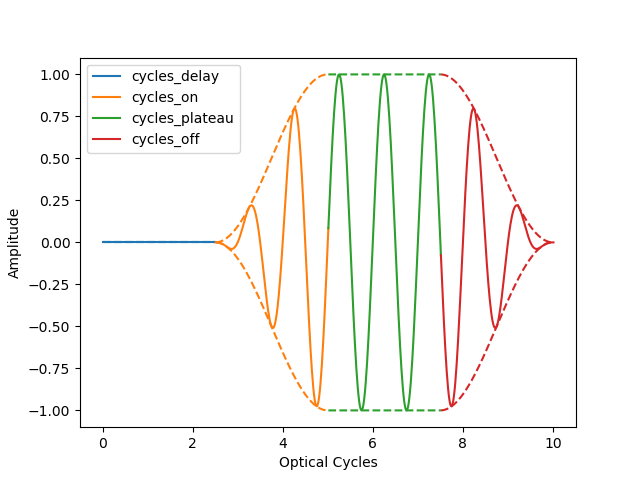
\includegraphics[width=0.7\textwidth]{Pulse.png}
\caption{A graphical depiction of the various laser parameters described in Sec.~\ref{sub:parameters}. The dotted lines show the laser envelope and the solid lines are the vector potential. The various colors show what regions are effected by the various laser parameters. Depicted is a sin$^2$ pulse.}
\label{fig:pulse}
\end{figure}

The code itself supports slightly more general pulse shapes than the standard sine squared or Gaussian pulse. The code allows for the pulse to be delayed before starting using the cycles\_delay parameter, ramped on for a period of time using the cycles\_on parameter, then held at its max intensity for using cycles\_plateau, and ramped off using the cycles\_off parameter. See Fig.~\ref{fig:pulse} for a graphical representation of the parameters. This allows for the creation of most pulses. The code also supports multiple pulses that can be controlled independently of each other. The on and off ramps can either be a sin$^n$ or Gaussian shape. You can mixed powers of sine (\textbf{must be even}) in a single pulse, however, if Gaussian is chosen both ramps are Gaussian though they can half different widths. For the Gaussian pulses, the code propagates for 5 times the full width half max (FWHM) on the ramp on and off. This brings the Gaussian close to zero since a Gaussian is never truly zero. This may want to be tested further at some point, though it will have a minimal impact on the physics and a significant impact on runtime if increased/decreased.

Using flat top pulses (cycles\_plateau $>$ 0) can clean up many results, however, they are extremely difficult to produce experimentally for pulses less than a picosecond. Due to this, reviewers may have issues with these pulses. Just something to be aware of.

\subsubsection{Experiment type} % (fold)
\label{ssub:experiment_type}
TODO
\begin{itemize}
  \item ``default''
  \item ``File''
  \item ``streaking''
\end{itemize}
% subsubsection experiment_type (end)

% subsection lasers (end)

% subsection potentials (end)

\section{Build System} % (fold)
\label{sec:build_system}
The build system changes from time to time. For the most up to date version, see the README in the root directory of this repository.
% section build_system (end)

\section{Input} % (fold)
\label{sec:input}

For the code, the only thing that needs to be in the directory is the ``input.json'' file. This will describe the laser, atomic/molecular target, and various other things required for the code to run. This section will go through what each parameter means and a list of options for each parameter when applicable.

The input files are in the json format. This formate is standardized, however, missing or extra commas, brackets, braces, ect.\ can be tricky to track down if you are not familiar with the json format. \textbf{Please take the time to learn json now. You will thank yourself later.}

\textbf{Make sure to use ASCII characters, copy and paste could cause issues!}

\subsection{Example File} % (fold)
\label{sub:example_file}
The following is an input file for simulating an 8 cycle, 800nm, sine squared pulse incident on atomic Hydrogen. This will produce a well converged High Harmonic Spectrum, though it may take a few hours to run. For a faster simulation that will be close to right, you can increase ``delta\_x\_max'' and ``delta\_x\_min'' to a larger number (say 0.5). You will need to do this for both dimensions.

\textbf{Make sure to use ASCII characters, copy and paste could cause issues!}

(current versions of example files can be found in the ``example'' directory)
\begin{verbatim}
{
  "alpha": 0.0,
  "coordinate_system": "Cylindrical",
  "delta_t": 0.1,
  "dimensions": [
    {
      "delta_x_max": 0.1,
      "delta_x_max_start": 4.0,
      "delta_x_min": 0.1,
      "delta_x_min_end": 4.0,
      "dim_size": 100.0
    },
    {
      "delta_x_max": 0.1,
      "delta_x_max_start": 4.0,
      "delta_x_min": 0.1,
      "delta_x_min_end": 4.0,
      "dim_size": 200.0
    }
  ],
  "field_max_states": 0,
  "free_propagate": 0,
  "gauge": "Velocity",
  "gobbler": 0.9,
  "laser": {
    "experiment_type": "default",
    "pulses": [
      {
        "cep": 0.0,
        "cycles_delay": 0.0,
        "cycles_off": 4.0,
        "cycles_on": 4.0,
        "cycles_plateau": 0.0,
        "ellipticity": 0.0,
        "energy": 0.057,
        "helicity": "left",
        "intensity": 1e14,
        "polarization_vector": [
          0.0,
          1.0,
          0.0
        ],
        "power_off": 2.0,
        "power_on": 2.0,
        "poynting_vector": [
          0.0,
          0.0,
          1.0
        ],
        "pulse_shape": "sin"
      }
    ]
  },
  "num_electrons": 1,
  "order": 2,
  "propagate": 1,
  "restart": 0,
  "sigma": 3.0,
  "start_state": {
    "amplitude": [
      1.0
    ],
    "index": [
      0
    ],
    "phase": [
      0.0
    ]
  },
  "state_solver": "SLEPC",
  "states": 5,
  "target": {
    "name": "H",
    "nuclei": [
      {
        "SAE": {
          "a": [
            0.66294407
          ],
          "b": [
            4.073942
          ],
          "c0": 1.0,
          "r0": 2.353059,
          "z_c": 1.0
        },
        "location": [
          0.0,
          0.0,
          0.0
        ],
        "z": 1.0
      }
    ]
  },
  "tol": 1e-10,
  "write_frequency_checkpoint": 1000,
  "write_frequency_eigin_state": 1000,
  "write_frequency_observables": 1
}
\end{verbatim}
% subsection example_file (end)

\subsection{Parameters} % (fold)
\label{sub:parameters_input}
The following is my attempt as describing what each parameter does. Each parameter is a subsubsection and they should come in the order of the example input file in Sec~\ref{sub:example_file}. Sub section names for nested parameters include a ``-'' to show that the parameter is either part of a list or dictionary of a different parameter. This is shown in Sec~\ref{ssub:dimensions-dim_size} as ``dim\_size'' is a sub parameter of the ``dimensions'' parameter.  Some of the parameters have extra descriptions that are critical to reproduce results from other codes. This may lead to some lengthy discussion that may not be useful for all users. If you have questions on particular parameters or more general questions, let me know.

\textbf{Make sure to use ASCII characters, copy and paste could cause issues!}

\subsubsection{alpha}
alpha is the soft core parameter described in Sec~\ref{ssub:soft_core_like}. A floating point number can be input, and a value of 0.0 leads to the standard Euclidean distance $r=\sqrt{x^2+y^2+\cdots}$. It is used in the Coulomb (Hydrogen like) potentials. It is also used for any $r$ that comes in the denominator of the Single Active Electron (SAE) Potentials in Sec~\ref{ssub:single_active_electron}. Any $r$ that comes in the numerator is the standard Euclidean distance. The soft core takes the mathematical form of
\begin{equation}
  r_{soft} = \sqrt{r^2 + \alpha^2}
\end{equation}
where $r$ is the standard Euclidean distance.

\subsubsection{coordinate\_system}
This describes the available coordinate systems available. Current list of available coordinate systems is (make sure to use ASCII quotes, don't just copy and paste)
\begin{itemize}
  \item ``Cartesian''
  \item ``Cylindrical''
  \item ``RBF'' (beta)
\end{itemize}
The ``Cartesian'' coordinate system supports 1-3 dimensions with up to 2 electrons with any laser polarization that can be described in that number of dimensions. Though 2 electron calculations are computationally limiting. ``Cylindrical'' is a discretization in cylindrical coordinates for linear polarization on atoms or aligned linear molecules. It is 2 dimensional ($\rho$ and $z$) and runs much faster than a 3D simulation would. The ``RBF'' code is very much in beta testing and requires and external package. Only those wishing to get their hands dirty developing the method further should use this code. Talk to me if this is you.

\subsubsection{delta\_t}
delta\_t is the time step used in the simulation in atomic units (floating point number). Time steps in the range of 0.05 to 0.1 are typically sufficient for a simulation, however, one must run a convergence test non the particular observable you're interested in.

\subsubsection{dimensions}
\label{ssub:dimensions}
dimensions is a list of json objects (also known as dictionaries). Each dictionary provides the size of a new dimension. In the Cartesian coordinate system, the dimensions are added in the order x, y, z. If only 2 dictionaries are included, a 2D simulation is preformed. For Cylindrical coordinates the dimensions are added in the order $\rho$ and $z$.

\textbf{Note}: Each dimension can have a minimum grid spacing and a maximum grid spacing with a sine squared ramp connecting them. This appears to work for ground state calculations, however, time propagation can have issues. Take extra care if you wish to use this feature. If ``delta\_x\_min'' $=$ ``delta\_x\_max'' are the same value, the code has been well tested and will produce good results (you just have to get past the error checks by moving ``delta\_x\_max\_start'' and ``delta\_x\_min\_end'' away from the boundaries of your grid).

\subsubsection{dimensions - delta\_x\_max}
delta\_x\_max is the max grid spacing in atomic units (outside edge of the grid). This is useful to describe highly excited states and outgoing wave packets, though it is not 100\% stable. Set equal to delta\_x\_min to use the well tested code. Typical values for converged calculations on a uniform grid are less than or equal to 0.1. See the note in Sec~\ref{ssub:dimensions} for more details on nonuniform grid.

\subsubsection{dimensions - delta\_x\_max\_start}
delta\_x\_max\_start is the distance from the origin that the delta\_x\_max is used to increase the grid size. See the note in Sec~\ref{ssub:dimensions} for more details on nonuniform grid.

\subsubsection{dimensions - delta\_x\_min}
delta\_x\_min is the min grid spacing in atomic units (outside edge of the grid). This is useful to describe highly excited states and outgoing wave packets, though it is not 100\% stable. Set equal to delta\_x\_max to use the well tested code. Typical values for converged calculations on a uniform grid are less than or equal to 0.1. See the note in Sec~\ref{ssub:dimensions} for more details on nonuniform grid.

\subsubsection{dimensions - delta\_x\_min\_end}
delta\_x\_min\_end is the distance from the origin that the sine squared ramp up between delta\_x\_min and delta\_x\_max begins. See the note in Sec~\ref{ssub:dimensions} for more details on nonuniform grid.

\subsubsection{dimensions - dim\_size}
\label{ssub:dimensions-dim_size}
dim\_size is the total size of the dimension in atomic units. For all Cartesian and the $z$ axis in Cylindrical, the grid will go from -dim\_size/2 to dim\_size/2. For the $\rho$ dimension in Cylindrical, the grid will go from 0 to dim\_size.

\subsubsection{field\_max\_states}
field\_max\_states allows for the peak of the electric field or vector potential to be used for eigenstate calculations. Utilizing this parameter is still in beta. Testing is required if this parameter is not set to 0. The following values can be set
\begin{itemize}
  \item ``0'' Field free (standard use case)
  \item ``1'' Field max (still in beta)
\end{itemize}

\subsubsection{free\_propagate}
free\_propagate is the number of time steps the wavefunction is propagated after the last laser ``finishes'' (integer). Total free propagation is delta\_t * free\_propagate in atomic units.

\subsubsection{gauge}
gauge allows for calculation to be done in Velocity and Length gauge and runtime differences are negligible in the cases I've tested. Both should produce the same answer when fully converged. The options are
\begin{itemize}
  \item ``Velocity''
  \item ``Length''
\end{itemize}

\subsubsection{gobbler}
This sets the size of the exterior complex scaling (ECS) potential (Sec~\ref{ssub:exterer_complex_scaling}) which absorbs outgoing wavepackets. A value of 0.9 means that 90\% of the grid is normal and the outer 5\% on each side contains an ECS potential.

\subsubsection{laser}
The laser parameter is a dictionary that contains the particular laser being used in the calculation.

\subsubsection{laser - experiment\_type}
The experiment\_type is how the laser is being used. The options are
\begin{itemize}
  \item ``default''
  \item ``File''
  \item ``streaking''
\end{itemize}
Below is documentation for ``default''. Details on the others can be found in Sec~\ref{ssub:experiment_type}.

\subsubsection{laser - pulses}
pulses is a list of dictionaries used to describe a pulse. Each component inside a single pulse is in the units of that pulse such as the length of a single cycle is based on the frequency of that particular pulse.

\subsubsection{laser - pulses - cep}
cep is the carrier envelope phase (CEP) which is $\phi_A$ in Eq.~\ref{eq:afield}. It is in units of 2$\pi$, so a value of 0.5 gives $\phi_A=\pi$. The CEP is defined off of $t_0$ which is defined at the end of cycles\_on (peak of laser field/beginning of the plateau).

\subsubsection{laser - pulses - cycles\_delay}
cycles\_delay is the number of cycles until the ramp up of the pulse begins. See Fig.~\ref{fig:pulse} for a graphical representation.

\subsubsection{laser - pulses - cycles\_off}
cycles\_off is the number of cycles that ramps the pulse back to zero. See Fig.~\ref{fig:pulse} for a graphical representation. Note that this is the full size for ``sin'' envelopes and the FWHM for ``Gaussian''. The ``Gaussian'' shapes are propagated for 5 times the cycles\_on to allow for the envelope to approach zero.

\subsubsection{laser - pulses - cycles\_on}
cycles\_on is the number of cycles that ramps the pulse from zero to its max value. See Fig.~\ref{fig:pulse} for a graphical representation. Note that this is the full size for ``sin'' envelopes and the FWHM for ``Gaussian''. The ``Gaussian'' shapes are propagated for 5 times the cycles\_on to allow for the envelope to approach zero.

\subsubsection{laser - pulses - cycles\_plateau}
cycles\_plateau is the number of cycles the pulse remains at its max value. See Fig.~\ref{fig:pulse} for a graphical representation.

Using flat top pulses (cycles\_plateau $>$ 0) can clean up many results, however, they are extremely difficult to produce experimentally for pulses less than a picosecond. Due to this, reviewers may have issues with these pulses. Just something to be aware of.

\subsubsection{laser - pulses - ellipticity}
ellipticity is the ratio of the minor over major axis for the laser polarization. 0.0 gives linear polarization and 1.0 gives circular polarization.

\subsubsection{laser - pulses - energy}
energy provides the central frequency ($\omega_A$) in Eq.~\ref{eq:afield}. Given in atomic units (800nm $\approx$ 0.057a.u.). Note that the frequency shift (Eq.~\ref{eq:fshift}) described in Sec~\ref{sub:lasers}should be accounted for when pulses are around 15 optical cycles or less.

\subsubsection{laser - pulses - helicity}
helicity is the handedness of elliptical and circular polarized lasers. It take the values of:
\begin{itemize}
  \item ``left''
  \item ``right''
\end{itemize}

\subsubsection{laser - pulses - intensity}
intensity is the peak intensity of the laser field. It is given in W/cm$^2$. Typical values are $10^{12}$ to $10^{15}$. Easiest to provide in the from $2e12$ for $2*10^{12}$, though it can be written out with all the zeros if one wishes.

\subsubsection{laser - pulses - polarization\_vector}
polarization\_vector is a list that defines the direction of the major axis of the laser. It is normalized after being read in to avoid intensity scaling issues. The order of dimensions is the same as the coordinate system defined in Sec.~\ref{ssub:dimensions}.

\subsubsection{laser - pulses - power\_off}
power\_off is the power a ``sin'' envelope function is raised to on the ramp off portion of the pulse scaled by cycles\_off. The value must be an even power giving the envelope the form $\sin^{power\_off}$.

\subsubsection{laser - pulses - power\_on}
power\_on is the power a ``sin'' envelope function is raised to on the ramp on portion of the pulse scaled by cycles\_on. The value must be an even power giving the envelope the form $\sin^{power\_on}$.

\subsubsection{laser - pulses - poynting\_vector}
poynting\_vector defines the direction of propagation of the laser. When combined with the polarization\_vector and helicity, the coordinate system for the laser has been set. It is normalized after being read in to avoid intensity scaling issues. The order of dimensions is the same as the coordinate system defined in Sec.~\ref{ssub:dimensions}.

\subsubsection{laser - pulses - pulse\_shape}
pulse\_shape gives the ramp functions for the pulse. They are either sin$^n$ (where $n$ is set using power\_on and power\_off) or Gaussian. The values it takes are
\begin{itemize}
  \item ``sin''
  \item ``gaussian''
\end{itemize}

\subsubsection{num\_electrons}
num\_electrons is the number of electrons in the simulation. Having more than one electron should work but has not been throughly tested. Ask for 3 or more electrons for an easter egg.

\subsubsection{order}
order is the order of finite difference used. Only 2nd order appears to work, however, and even order seams to work for ground state calculations. I recommend just leaving it set to 2.

\subsubsection{states}
states is the number of bound states of your potential you would like to calculate. It is also the number of states that are used to calculate populations in the code and projected out for removing the bound state population when calculating photoelectron spectra. This is a number, except when using the ``Power'' method as a state\_solver. Then is it a list of dictionaries with target energies provided. Here is an example:
\begin{verbatim}
"states": [{"energy": -0.5}, {"energy": -0.125}]
\end{verbatim}

\subsubsection{start\_state}
start\_state is a dictionary that defines the initial conditions for time propagation. The initial state $\Psi$ is given by
\begin{equation}
  \Psi = \sum\limits_n a_n e^{i\phi_n} \psi_n^{idx}
  \label{eq:start_state}
\end{equation}
$a_n$ is the amplitude, $psi_n$ is the bound state, $\phi_n$ is the phase, $n$ is the index into the ``amplitude'', ``index'', and ``phase'' arrays, and $idx$ is the index into the bound state data file given in the ``index'' array. The initial wavefunction is normalized to one after being read in, so the amplitude array's values are only relative amounts.

\subsubsection{start\_state - amplitude}
amplitude defines the $a_n$ in Eq.~\ref{eq:start_state} where $n$ is the index into this array. The initial wavefunction is normalized to one after being read in, so the amplitude array's values are only relative amounts.

\subsubsection{start\_state - index}
index is the $idx$ wavefunction in the bound state file being used. It takes the value of $idx$ in Eq.~\ref{eq:start_state} where $n$ is the index into this array. Note that the bound state file wavefunctions may have a random phase.

\subsubsection{start\_state - phase}
phase is the value of $\phi_n$ in Eq.~\ref{eq:start_state} where $n$ is the index into this array. Note that the bound state file wavefunctions may have a random phase. If relative phase is important to your system take extra care when setting this.

\subsubsection{state\_solver}
state\_solver it the method used to calculate ground states. ``SLEPC'' or ``File'' are the recommended modes of operation. All of the options are
\begin{itemize}
  \item ``File''
  \item ``SLEPC''
  \item ``Power''
  \item ``ITP'' (deprecated)
\end{itemize}

``File'' will read from the file given in ``target - name'' with a ``.h5'' extension added to it. This allows for the same bound state file to be used by many calculations.

``SLEPC'' utilized the SLEPc library to calculate eigen states. It uses the default SLEPc solver (currently Krylov Schur) though this can be changed by added the command line argument ``-eps\_type $<$method$>$'' when running the code. See the SLEPc for more information on how to do this.

``Power'' is the inverse shifted power method with target energies given by the ``states'' parameter. See ``states'' for an example on how to provide target energy values.

``ITP'' is imaginary time propagation. This is no longer supported as much better methods have been implemented, though it does lead to an easter egg.

\subsubsection{target}
target is how you define the potential (or target) in which you want to calculate bound states of or shine a laser on.

\subsubsection{target - name}
name is the name of the bound state file. It can also be used to provide a path to place/read from the file in a different folder. You should avoid spaces and punctuation in file names (follow good file naming practices). Note that the ``.h5'' is added inside the code, so it should not appear in this name.

\subsubsection{target - nuclei}
nuclei is a list that allows for nuclei to be placed at various places in space. Each can be coulomb or SAE (this may change later).


\subsubsection{target - nuclei - SAE}
SAE is used when z is set to 0, otherwise the SAE potential is ignored. This allows for SAE potentials from Brynn to be used. They take the form
\begin{equation}
  V(r, r_{soft}) = - \frac{c_0}{r_{soft}} - \frac{Z_c e^{-r_0 r}}{r_{soft}} - \sum_n a_n e^{-b_n r}
    \label{eq:SAE_target}
\end{equation}
where $r_{soft}$ is the soft core distance from the nuclei's location and $r$ is the euclidean distance form the nuclei's location.

\subsubsection{target - nuclei - SAE - a}
a is the $a_n$ value in Eq.~\ref{eq:SAE_target} where $n$ is the index into this array.

\subsubsection{target - nuclei - SAE - b}
b is the $b_n$ value in Eq.~\ref{eq:SAE_target} where $n$ is the index into this array.

\subsubsection{target - nuclei - SAE - c0}
c0 is the $c_0$ value in Eq.~\ref{eq:SAE_target}.

\subsubsection{target - nuclei - SAE - r0}
r0 is the $r_0$ value in Eq.~\ref{eq:SAE_target}.

\subsubsection{target - nuclei - SAE - z\_c}
z\_c is the $Z_c$ value in Eq.~\ref{eq:SAE_target}.

\subsubsection{target - nuclei - location}
location is a list that corresponds to the nuclei center. The distances $r$ and $r_{soft}$ are calculated from it. The order of dimensions is the same as the coordinate system defined in Sec.~\ref{ssub:dimensions}.

\subsubsection{target - nuclei - z}
z is the value of z in a coulomb like potential (Ea.~\ref{eq:coulomb}. If set to 0, the SAE potential is used otherwise the SAE potential is ignored. The potential is explicitly written as
\begin{equation}
  V(r_{soft}) = - \frac{z}{r_{soft}}
    \label{eq:coulomb}
\end{equation}
where $r_{soft}$ is the soft core distance from the nuclei's location.

\subsubsection{tol}
tol is used whenever a convergence tolerance is needed in the code. The only place I remember is for the eigen state calculations. A value of $1e-10$ is a good starting point.

\subsubsection{write\_frequency\_checkpoint}
write\_frequency\_checkpoint is the number of time steps between writing checkpoint files that allow the code to restart. Setting this to small can lead to massive data files. If it is to large, the code may crash before a checkpoint is written to disk. Typically you want a restart file written ever 20mins to a few hours of runtime depending on the size of the simulation. If you would like to make a video of the simulation, this can be set to a small value assuming you have the disk space.

\subsubsection{write\_frequency\_eigin\_state}
write\_frequency\_eigin\_state is the number of iterations between making convergence/writing to standard out checks when using the power method. Add ``-eps\_monitor'' to the run line in the bash script to monitor SLEPC calculations.

\subsubsection{write\_frequency\_observables}
write\_frequency\_observables is the number of time steps between writing calculating observables such as dipole, dipole acceleration, norm, ecs population, ect. I recommend leaving this set to 1 as it is not that time consuming in the current version of the code.
% subsection parameters(end)

% section input (end)



\section{Classes} % (fold)
\label{sec:classes}

The classes used in this code are written so they can be tested independently. Therefore, all classes that depend on other classes require those classes to be passed into the constructor. The developer is responsible to not delete these classes until other dependent classes are deleted.

For the most part, the classes do what you would expect. However, there are small deviations like the HDF5Wrappers writing the Parameters to the file rather than the other way around. This is done to enable restarts to not delete old datasets.

\subsection{PETSCWrapper} % (fold)
\label{sub:petscwrapper}
This class takes care of setting up SLEPC, PETSC, and MPI. It comes first so that the finalize calls are made once every other class has cleaned up after its self.
% subsection petscwrapper (end)

\subsection{ViewWrapper} % (fold)
\label{sub:viewwrapper}
This class wraps the HDF5 interface that PETSC supplies. It is used for dumping the wavefunctions to disk.
% subsection viewwrapper (end)

\subsection{Parameters} % (fold)
\label{sub:parameters}
This class holds the input file information and will be used by all other classes. It depends on a json parser (https://github.com/nlohmann/json) and reads inputs in json format. For more information about input parameter definitions and how they are used, see Section~\ref{sec:input}. This class is mainly used as a data structure. That being said, it does provided tools to validate various input parameters to limit user error. It is also used to convert the various laser input styles to the ``default'' style that the Pulse class needs to create the laser fields.

The code currently reads the input files from every processor in use. This hasn't been an issue running on upwards of 6,000 processors, but it should be changed at some point.

% subsection parameters (end)

\subsection{HDF5Wappers} % (fold)
\label{sub:hdf5wappers}
IO for this code is done using HDF5 files. HDF5 files provide the ability to utilize parallel file systems, generate self describing data files, and write compressed data. With these advantages, it becomes slightly more difficult to write data. To alleviate this issues, this class provides tools for writing to HDF5 files in a straight forward way.

Writing multidimensional arrays is difficult in HDF5. To avoid the added headache, one denominational arrays with the access pattern of
\begin{equation}
	array[x+y*nx] = array[x][y]
\end{equation}
and
\begin{equation}
	array[x+y*nx+z*nx*ny] = array[x][y][z]
\end{equation}
and so on. Note that the ordering flips when using python to visualize the data due to the c vs fortran ordering of arrays. Be sure to pay close attention to axis labels to make sure the data is orientated correctly.
% subsection hdf5wappers (end)

\subsection{Pulse} % (fold)
\label{sub:pulse}
Pulse handles creating and storing various parts of the pulse. Much of the functionality is private rather than public to prevent accessing data that is not allocated. Since storing each individual pulse is only useful until it is printed to a file, it is deallocated inside the constructor. The result is a much more efficient use of memory, and protection from accessing garbage arrays. See Section~\ref{sec:input} on how to define pulses.
% subsection pulse (end)

\subsection{Hamiltonian} % (fold)
\label{sub:hamiltonian}
We are interested in solving the Solving the Time-Dependent Sch\"{o}dinger Equation for atoms and molecules.
\begin{equation}
    i\frac{\partial}{\partial t}\psi(x,t) = \hat{H}\psi(x,t)
\end{equation}
Which leads to a Hamiltonian of
\begin{equation}
    \hat{H} = \sum_{e}\left(\frac{\hat{\mathbf{p}}^2_e}{2} - \frac{\mathbf{A}(t) \cdot \hat{\mathbf{p}}_e}{c} - \sum_{n} \frac{Z_n}{r_{e,n}}\right) + \sum_{e_1 < e_2}\frac{1}{r_{e_1, e_2}}
\end{equation}
The full problem is pretty much impossible to solve for 3 or more electrons. For a two electron atom (He like), we have the following Hamiltonian.
\begin{equation}
  \hat H = \frac{\hat{p_1}^2}{2} + \frac{\hat{p_2}^2}{2} - \frac{\vec{A} \cdot (\hat{p_1}+\hat{p_2})}{c} - \frac{Z}{x_1} - \frac{Z}{x_2} + \frac{1}{r_{12}}
\end{equation}

The Hamiltonian class takes the input file and defines the appropriate matrix to operate on our wave function. There is tons of index gymnastics going on in this class. Creation of the Hamiltonian is currently around 30\% of the total run time of a simulation. This code has some low hanging optimizations like storing the time independent Hamiltonian. This should be the next priority in optimizations. For a full explanation the numeric methods we use and justification for various tools, see Section~\ref{sec:theory}.

% subsection hamiltonian (end)

\subsection{Simulation} % (fold)
\label{sub:simulation}
The simulation class implements various propagation and eigen state calculations. It then utilized every other class to provide the appropriate IO and behavior at various points in the simulation.
% subsection simulation (end)

% section classes (end)


\section{Testing} % (fold)
\label{sec:testing}
There is very little testing used in this code. If you would like to work on this or notices something is wrong. Please let me know.
% section testing (end)

\section{Wish list} % (fold)
\label{sec:wish_list}
\begin{itemize}
    \item Faster algorithm (radial code, numerical basis, non uniform grid, RBF, ect.)
    \item Free propagation support (Density Matrix for bound states)
    \item New features (fast two electron code)
    \item Moving nuclei (classical and quantum mechanical)
\end{itemize}
% section wish_list (end)

\section{Supporting works} % (fold)
\label{sec:supporting_works}

\subsection{Posters} % (fold)
\label{sub:posters}

% subsection posters (end)
\subsection{Talks} % (fold)
\label{sub:talks}

% subsection talks (end)
\subsection{Papers} % (fold)
\label{sub:papers}

% subsection papers (end)
% section supporting_works (end)
\section{Contributors} % (fold)
\label{sec:contributors}
The following people have contributed to this code. No particular order is used.
\begin{itemize}
  \item Joel Venzke
  \item Cory Goldsmith
\end{itemize}
% section contributors (end)
\end{document}